
\documentclass[bachelor,print,msfonts]{xduthesis}
%\documentclass[bachelor,print]{xduthesis}

\usepackage{listings}
\usepackage{overpic}
\usepackage{algorithm}
\usepackage{algorithmicx}
\usepackage{algpseudocode}
\usepackage{booktabs}
\usepackage{colortbl}
\usepackage{multirow}
\usepackage{pgfplots}
\usepackage{mathtools}
\newtagform{EueTag}{式~(}{)}
\usetagform{EueTag}
\lstset{language=TeX, basicstyle=\ttfamily}

\newcommand{\figref}[1]{图\ref{#1}}
\newcommand{\sArt}{state-of-the-art}
\newcommand{\wyh}[1]{{\textcolor{blue}{#1}}}
\newcommand{\secref}[1]{Sec. \ref{#1}}
\newcommand{\tabref}[1]{Tab.~\ref{#1}}
\newcommand{\thudot}[1]{}
\renewcommand{\emph}[1]{\texttt{#1}}

\floatname{algorithm}{算法}
\renewcommand{\algorithmicrequire}{\textbf{输入:}}
\renewcommand{\algorithmicensure}{\textbf{输出:}}

\newcommand{\mypara}[1]{\paragraph{#1.}}

\begin{document}

%%%%%%%%%%%%%%%
%% 论文前置部分
%%%%%%%%%%%%%%%
\frontmatter

% 论文相关信息(封面)
\classid{1513018}
\studentid{15130188018}

\cschool{计算机科学与技术学院}
\ctitle{基于多任务学习的文本\\表示方法研究}
\cauthor{孙天祥}
\cmajor{软件工程}
\csupervisor{刘西洋~教授}

% 中英文摘要声明
\begin{cabstract}
	文本表示是自然语言处理的必要任务,表示方法的好坏对于模型性能至关重要。为得到泛化能力强的文本表示,近年来多任务学习被广泛应用在各大自然语言处理任务中,通过联合学习多个相关任务来共享任务间的知识,从而提升模型在各个任务上的表现。
	
	近期,一种新型的神经网络模型Transformer因其在机器翻译和迁移学习等方面取得的巨大成功开始在自然语言处理领域流行。然而,之前的工作大都在卷积网络和循环网络上研究多任务学习的共享结构,目前还很少有工作探究Transformer上的多任务共享架构。本文在Transformer上探索了句子级的多任务文本表示方法:首先设计了两种传统的硬共享结构,接着提出了两种逐层共享结构,能够在每一层根据输入动态地抽取其他任务的特征来形成任务特定表示。我们在16个情感分析任务上进行了实验,对比单任务模型,四种多任务模型的准确率均取得了较大提升,其中,本文提出的两种逐层共享结构均超越了传统共享结构。
	
	最后,我们对模型进行了实例分析,总结了现有工作,并展望了未来多任务学习在自然语言处理以及深度学习的发展。
\end{cabstract}


\begin{ckeywords}
	自然语言处理\ \ \ \ \ \ 表示学习\ \ \ \ \ \ 多任务学习
\end{ckeywords}

%\cthesistype{应用基础技术}


\begin{eabstract}
	Language representation is an essential task for natural language processing(NLP). To learn general representation, multi-task learning(MTL) methods, which allow models to share knowledge in related tasks by joint learning, are applied to many NLP tasks.
	
	Recently, Transformer, a novel neural network based on self-attention mechanism, has become popular in NLP due to its great success in machine translation and transfer learning. Most of previous works focus on designing multi-task sharing scheme for convolutional networks and recurrent networks. However, there is few discussion on multi-task learning in Transformer. In this paper, we propose 4 sentence-level multi-task transformer architectures: two traditional hard sharing architectures and two layerwise sharing architectures, which can dynamically combine features of related tasks and generate task-specific representation based on the input at each layer. We conduct experiments on 16 sentiment analysis tasks. Our 4 multi-task transformers consistently outperform transformers trained with single task. Besides, the proposed layerwise sharing architectures achieve better accuracy than traditional architectures.
	
	Finally, we conduct case study for our proposed model, summarize the existing works, and look forward to the future development of multi-task learning in natural language processing and deep learning.
	
	
\end{eabstract}


\begin{ekeywords}
	Natural Language Processing\ \ \ \ Deep Learning\ \ \ \ Multi-Task Learning
\end{ekeywords}

%\ethesistype{Applied Basic Technology}

% 生成论文的封面、声明页、中英文摘要
\makecover

% 论文目录
\tableofcontents

%%%%%%%%%%%%%%%
%% 论文正文
%%%%%%%%%%%%%%%
\mainmatter

\chapter{绪论}
\label{cha:intro}
本章首先介绍基于深度学习的自然语言处理的研究背景,阐述在该背景下多任务学习的研究价值及意义。接着简要介绍自然语言处理和多任务学习的研究进展,并指出目前存在的问题。然后介绍本文的研究内容及目标,并概括了本文工作的创新之处。本章的最后给出了论文的主要内容和章节安排。

\section{研究背景及意义}
1950年,阿兰·图灵(Alan Turing)提出了著名的\emph{图灵测试}\footnote{图灵测试是指,一个人在不接触对方的情况下,通过某种方式和对方进行一系列的问答。若在相当长时间内,他无法根据问答的情况判断对方是人还是机器,那么可以认为该机器具备智能。},直接推动了人工智能从哲学探讨的层面上升到科学研究。随后不久,在1956年举办的达特茅斯会议上,\emph{人工智能}的概念被正式提出,John McCarthy将这一新兴领域的研究目标定义为:“让机器的行为看起来像人类所表现出来的智能行为一样”。自1956年至今的六十余年中,研究人员尝试了多种方法来实现这一愿景,人工智能领域也随着这些方法的成功与失败经历了数次热潮与低谷。近年来,随着数据量的增加和算力的增强,以神经网络为代表的\emph{深度学习}异军突起,在语音识别\cite{DBLP:conf/asru/MikolovDPBC11}\cite{DBLP:conf/apsipa/LiHYW13}、计算机视觉\cite{DBLP:journals/cacm/KrizhevskySH17}\cite{DBLP:journals/pami/FarabetCNL13}\cite{DBLP:conf/nips/TompsonJLB14}等众多应用场景中取得了巨大突破,也为自然语言处理领域带来了深刻的变革。

自然语言,即文明发展过程中自然形成的语言,是最能体现人类智慧和文明的产物。\emph{自然语言处理}(Natural Language Processing, NLP)被很多人认为是“人工智能皇冠上的明珠”,致力于使用计算机技术处理、理解和生成人类语言。随着深度学习技术的发展,越来越多的研究者开始使用深度学习的技术解决自然语言处理中的难题,在很多任务上远远超越了之前的传统方法\cite{DBLP:journals/jmlr/CollobertWBKKK11}\cite{DBLP:conf/emnlp/BordesCW14}\cite{DBLP:conf/acl/JeanCMB15}\cite{DBLP:conf/nips/SutskeverVL14}。

然而,对NLP问题的研究常常被划分为多个任务,如命名实体识别、阅读理解、机器翻译等。目前一般的做法是为当前关注的某一个任务设计特定的神经网络模型,在此单一任务及数据集上进行训练。遗憾的是,这样设计出来的模型常常具有较大的局限性,在某个数据集上表现优秀的模型可能在另一个数据集上就会表现很差,即使这两个数据集来自同一任务。并且,由于NLP任务及数据集众多,一时之间各种神经网络结构层出不穷。深度学习刚刚帮助人们从“特征工程”中脱离出来,很快又陷入了所谓的网络“结构工程”。同时,这也将模型限制在了特定领域,难以发展出更为通用的智能系统。

为解决这一问题,很多研究人员转而寻求泛化能力更加强大、能够提取数据更一般性的特征表示的模型,而不是为每一个新的任务甚至数据集设计新的模型。很快,人们发现通过迁移学习和多任务学习能够得到这样的模型。事实上,迁移学习和多任务学习能够有效的原因都在于模型参数共享,或者说知识共享。其中,迁移学习的主要形式就是预训练一个较为通用的模型,再在目标任务和数据集上进行微调。在计算机视觉领域,在ImageNet\cite{DBLP:conf/cvpr/DengDSLL009}这样的大规模图像分类数据集上预训练的模型能够在很多图像分类任务上表现良好;在NLP领域,通过在大规模无标注文本上预训练一个语言模型也通常能够给各种下游任务带来很大收益\cite{DBLP:conf/naacl/PetersNIGCLZ18}\cite{radford2018improving}。这些发现表明,共享模型在其他任务上学习到的知识能够显著提升模型的性能。

在这一背景下,人们开始思考:是否可以训练单个模型来处理几乎所有的任务?要想得到这样的单一模型,几乎无可避免地需要借助多任务学习的方法。近年来,多任务学习被广泛地应用在自然语言处理领域中,在序列标注、文本分类、机器翻译等多个经典NLP任务上都取得了令人鼓舞的效果。随着多任务学习的引入,人们发现很多NLP任务可以归纳为统一的模型范式,如问答范式\cite{mccann2018natural}、分类范式\cite{radford2018improving}\cite{devlin2018bert}。同时,越来越多的研究者开始关注模型在多任务上的表现,出现了decaNLP\cite{mccann2018natural}、GLUE\cite{DBLP:conf/emnlp/WangSMHLB18}等大规模多任务评测数据集。随着算法和评测基准的逐渐成熟,多任务学习模型的开发受到越来越多的研究者关注。同时也需要注意到,多任务学习的研究历史不过二三十年,对基于深层神经网络的多任务学习的研究甚至更短。因此,如何为各神经网络模型及任务设计合适的共享结构,仍然是亟待探索的问题。

\section{相关研究进展}

本节将简要介绍深度学习背景下的自然语言处理、多任务学习、深度学习以及它们相结合的研究进展及现状,并阐述了它们之间的联系以及目前存在的不足。

自然语言处理(NLP)是一门旨在使得计算机具备处理、理解和生成自然语言(人类语言)能力的学科。近年来,以神经网络为代表的深度学习在自然语言处理\cite{DBLP:journals/jmlr/CollobertWBKKK11}\cite{DBLP:conf/emnlp/BordesCW14}\cite{DBLP:conf/acl/JeanCMB15}\cite{DBLP:conf/nips/SutskeverVL14}中取得了广泛的成功。然而,不同于语音、图像等连续实值信号,自然语言是由离散的符号构成,这使其难以直接作为神经网络的输入。为解决这一问题,人们使用低维稠密向量来表征文本的语义信息\cite{DBLP:conf/nips/MikolovSCCD13}\cite{DBLP:conf/emnlp/PenningtonSM14},由于语义信息被分布到向量的各个维度,因此这种方法被称为分布式表示。随着分布式表示的引入,深度学习在自然语言处理领域得到了广泛的应用,卷积神经网络(CNN)、循环神经网络(RNN)相继被用于处理文本数据,近年来又提出了完全基于自注意力机制的全连接网络Transformer。这些神经网络的应用使得过去很多难以解决的NLP问题上取得了巨大进展。

事实上,文本的分布式表示的好坏对于模型的性能起着至关重要的作用。以分类任务为例,给定数据的一个好的表示,即使简单的线性分类器也能取得非常高的分类准确率\cite{tenney2018you}\cite{liu2019linguistic}。进入深度学习时代以来,自然语言处理领域中取得的许多突破都来自于对文本的通用表示方法的研究,如word2vec\cite{DBLP:conf/nips/MikolovSCCD13},ELMo\cite{DBLP:conf/naacl/PetersNIGCLZ18},BERT\cite{devlin2018bert}等。然而,相较于语音和图像数据,由于文本数据本身的离散性和歧义性,以及标注成本高、难度大等问题,如何得到一个好的文本表示仍然是自然语言处理领域的重大难题。

从机器学习的角度来看,一个好的表示方法除了能够在对应任务上表现良好,还应当具备良好的可迁移性与泛化能力,即能够在相似任务和新数据上获得较好的效果。在自然语言处理领域,常常使用\emph{多任务学习}(Multi-Task Learning, MTL)和\emph{迁移学习}(Transfer Learning)的方法来得到这样的文本表示\cite{devlin2018bert}\cite{DBLP:conf/icml/CollobertW08}。

对多任务学习较系统的研究可以追溯到1993年\cite{DBLP:conf/icml/Caruana93},它是指同时使用多个任务对模型进行训练,使其学习到数据的某种泛化表示,该表示能够同时解释这多个任务。多任务学习作为一种模型无关的技术,在很多传统的机器学习模型以及神经网络上都可以应用。特别地,由于神经网络易于扩展的特性,多任务学习在神经网络上的应用更为方便和灵活。

在过去的几年里,很多研究人员探索了多任务学习在CNN和RNN上的应用模式,验证了基于神经网络的多任务学习在文本表示上的有效性。Collobert等人\cite{DBLP:conf/icml/CollobertW08}使用一个简单的卷积网络来同时学习词性标注、语块标注、命名实体识别、语义角色标注、语义相似度、语言模型等多个任务,超越了使用单任务训练的效果。随着循环神经网络在NLP上的广泛应用,研究者开始基于循环网络构造多任务学习框架,在机器翻译\cite{DBLP:conf/acl/DongWHYW15}、文本分类\cite{DBLP:conf/ijcai/LiuQH16}\cite{DBLP:conf/acl/LiuQH17}、序列标注\cite{DBLP:conf/acl/SogaardG16}等常见NLP任务上均取得了成功。

多任务学习的一个关键问题在于如何设计一个高效的共享模式来允许模型共享多个任务的知识。上述提到的工作也大都致力于为所要解决的问题以及采用的网络结构来设计合适的共享模式,如硬共享模式、软共享模式、分层共享模式、共享-私有模式等。

同时,也有大量工作致力于使用迁移学习的范式来获取文本的通用表示,一般做法是利用语言模型\cite{DBLP:conf/naacl/PetersNIGCLZ18}\cite{radford2018improving}、机器翻译\cite{DBLP:conf/nips/McCannBXS17}或其他无监督任务\cite{devlin2018bert}来预训练一个可迁移的模型。并且,迁移学习与多任务学习本身并不互斥,因此可以同时利用二者的方法,使用多任务预训练迁移模型\cite{DBLP:conf/iclr/SubramanianTBP18},也可以在预训练得到的模型的基础上再使用多任务来微调\cite{liu2019multi}\cite{anonymous2018bam!}。

事实上,多任务学习和迁移学习本质上都是通过共享参数来迁移模型在不同任务中学习到的知识,并以此来提升泛化能力。因此,通常在迁移学习中效果很好的模型也可以应用在多任务学习中。近期,以Transformer为预训练网络结构得到的迁移模型GPT\cite{radford2018improving}和BERT\cite{devlin2018bert}在诸多自然语言处理任务上取得了极大的提升,这证明了Transformer强大的文本表示能力。然而,不同于CNN和RNN,目前还很少有工作研究多任务学习在Transformer上的应用模式,已有的少量工作也只是将最传统的多任务共享模式简单地应用在Transformer中\cite{liu2019multi}。

\section{本文研究内容}

本文试图在一定程度上填补目前多任务学习在Transformer结构下的研究空缺,探索基于Transformer的多任务共享模式,并通过实验比较几种多任务Transformer结构的效果。首先,本文考察了传统的硬共享模式在Transformer上的应用效果,然后,根据Transformer自身的结构特点设计了新的多任务架构。

在CNN及RNN结构中应用多任务学习通常是“纵向”的,如硬共享模式和分层共享模式,即在网络结构的某一层上堆叠任务特定层\cite{DBLP:conf/acl/SogaardG16}\cite{DBLP:conf/ijcai/ZhengCQ18}。这种架构蕴含着一个假设:存在某种通用的文本表示,特定的任务表示可以由该通用表示通过简单的变换得到。然而,这样的假设限制了能够同时学习的任务的多样性,难以处理弱相关任务及不同难度的任务。此外,任务特定层的位置通常需要根据任务特点来人为设定,这增大了多任务学习的应用难度。也有一些工作采用了“横向”共享的架构,如软共享模式和共享-私有模式,即允许模型使用其他任务的模型在同一层的隐状态\cite{DBLP:conf/ijcai/LiuQH16}\cite{DBLP:conf/cvpr/MisraSGH16}\cite{1705.08142},然而这些架构也存在两个问题:(1)通常需要为每个任务训练一个模型,参数量大且难以扩展;(2)各任务模型之间的信息交互难以控制。

而在Transformer中,可以很容易地在“横向”以记号的形式进行扩展,并且扩展的记号可以像普通单词一样与句子中的每个单词进行交互。同时,相比软共享、共享-私有模式等“横向”共享方法,这种共享结构只需增加少量参数。基于这一特性,本文给出了两种新型多任务共享模式:层级-隐式共享模式(L-I结构)和层级-显式共享模式(L-E结构)。在十六个文本分类数据集上进行的实验表明,本文提出的层级-隐式共享结构只需要增加0.5\%的参数量就可以提升约5\%的平均分类准确率。

此外,建模多任务之间的联系一直是多任务学习领域的研究重点。层级-显式共享结构可以直接利用注意力机制对任意任务之间的关系进行建模。并且,由于注意力机制的引入,本文的多任务Transformer结构具备良好的可解释性。对注意力得分矩阵的可视化为模型的预测结果提供了证据,展示了任务之间的交互关系。

\section{论文结构}

本文主要内容包括介绍已有的基于多任务学习的文本表示方法,几种新型的多任务文本表示模型及其实验结果,工作总结及对未来的展望。全文分为五个章节进行介绍,具体结构安排如下:

第~\ref{cha:intro}~章,介绍研究背景及意义,概括本文的研究内容。

第~\ref{cha:related_work}~章,介绍相关的理论基础及前沿进展。在~\ref{sec:dl}~节介绍深度学习的相关概念;在~\ref{sec:mtl}~节介绍基于神经网络的多任务学习;在~\ref{sec:nlp}~节介绍深度学习背景下自然语言处理的发展现状;在~\ref{sec:mtl4nlp}~节介绍多任务学习在自然语言处理中的应用。

第~\ref{cha:model}~章,详细描述本文设计的模型结构及实现细节。在~\ref{sec:tf}~节介绍Transformer的模型结构;在~\ref{sec:mtl_tf}~节设计了几种多任务Transformer架构;在~\ref{sec:imp}~节给出本文所使用的超参数设置以及实现细节。

第~\ref{cha:exp}~章,介绍实验相关的信息。在~\ref{sec:task}~节描述模型应用的具体任务;在~\ref{sec:ds}~节给出本文使用的各个数据集的有关信息;在~\ref{sec:results}~节对比了各模型在各数据集上的实验结果;最后在~\ref{sec:analysis}~节对模型进行了实例可视化分析。

第~\ref{cha:conclusions}~章,对本文的贡献和不足进行总结,回顾相关领域面临的机遇与挑战,并给出了未来的研究方向。


\chapter{相关工作}
\label{cha:related_work}
本文研究的内容包含了深度学习、多任务学习与自然语言处理三个主题,这里首先阐述这些主题之间的联系,接着分别介绍它们各自的相关概念与研究进展,最后介绍了三者交叉的一些重要研究工作。

我们利用深度学习与多任务学习来解决自然语言处理中的问题,具体的,即在深层神经网络中使用多任务学习来获得文本的泛化表示。从这一角度来看,深度学习与多任务学习是我们的工具,而自然语言处理为我们的应用场景。同时,深度学习与多任务学习都可以归为机器学习问题,而他们二者又有交叉,如图~\ref{fig:ml_dl_mtl}~所示。

\begin{figure}[htb]
	\centering
	\begin{tikzpicture}[scale=0.8]
	\draw (-4,3) rectangle (4,-3);
	\draw[draw = black] (-1.5,0) circle (2);
	\draw[draw = black] (1.5,0) circle (2);
	\node at (-2.8,2.5) {机器学习};
	\node at (-2,0) {深度学习};
	\node at (2,0) {多任务学习};
	\end{tikzpicture}
	\caption{机器学习、深度学习、多任务学习的关系}
	\label{fig:ml_dl_mtl}
\end{figure}

\section{深度学习}
\label{sec:dl}
近年来,深度学习(Deep Learning)发展十分迅速,在人工智能的很多子领域上取得了巨大成功,如语音识别\cite{DBLP:conf/asru/MikolovDPBC11}\cite{DBLP:conf/apsipa/LiHYW13}、计算机视觉\cite{DBLP:journals/cacm/KrizhevskySH17}\cite{DBLP:journals/pami/FarabetCNL13}\cite{DBLP:conf/nips/TompsonJLB14}、自然语言处理\cite{DBLP:journals/jmlr/CollobertWBKKK11}\cite{DBLP:conf/emnlp/BordesCW14}\cite{DBLP:conf/acl/JeanCMB15}\cite{DBLP:conf/nips/SutskeverVL14}等。

从要研究的问题来看,深度学习属于机器学习的一个分支,都是研究如何从有限个样例中通过某种算法总结出一般性规律或模式,并将其应用到新的未知数据上去。例如,通过机器学习或深度学习算法,可以根据历史病例总结出症状与疾病之间的规律,当遇到新的病人时可以利用算法总结出来的规律来帮助判断这个病人得了什么疾病\footnote{例子来源:《神经网络与深度学习》,邱锡鹏,\url{https://nndl.github.io}}。

同时,深度学习又与机器学习有很大的不同。从模型的构成来说,深度学习模型一般更加复杂,参数量更多。由于数据从输入到输出需要经过多个线性或非线性组件,信息传递路径较长,因此被称作深度学习。深度学习模型的一个最典型代表就是人工神经网络(Artificial Neural Network,ANN),下面简称神经网络。神经网络是一种受人脑神经系统启发的复杂数学模型,由神经元以及它们之间的连接组成。通过这些神经元的加工,原始数据从底层特征开始经过一道道加工逐渐得到抽象的高层语义特征。

总的来说,神经网络可以被看做一个包含大量参数的复合函数,该函数描述了输入和输出之间的复杂关系,因此可以被用于处理很多模式识别任务,如语音识别、图像识别等。形式化地,神经网络可以这样描述:
\begin{equation}
	y = \mathcal{F}(\mathbf{x} \mid \theta).
\end{equation}
其中,函数~$\mathcal{F}$~受参数~$\theta$~控制。

给定包含大量样例的集合,参数~$\theta$~可以通过随机梯度下降等优化算法得到,求解参数的优化过程就被称为\emph{学习过程},通过学习得到的参数被称为\emph{可学习参数},常简称为参数。还有一部分不可以被学习的参数,例如神经网络的层数,被称为\emph{超参数},意为控制参数的参数,超参数通常根据经验指定或根据实验效果来确定。

前面提到,参数学习需要一个包含大量样例的集合,该集合就是\emph{数据集}。在有监督学习中,每个样例一般包含输入~$\mathbf{x}$~和输出~$y$,输出也常被称为标签。其中,输入一般为一个向量,向量的每一个维度表示了样本的一个属性;输出一般为一个标量。包含~$n$~个样例的集合~$\mathcal{D} = \{ \mathbf{x}_i, y_i \}_{i=1}^n$~就是数据集。在实际使用时,数据集通常被划分为训练集、验证集(也叫开发集)和测试集。其中,用训练集来让算法学习参数,用验证集来调整算法的超参数,用测试集来衡量模型的优劣。

给定数据集~$\mathcal{D}$~和模型结构,即~$\mathcal{F}$的形式,优化算法可以得到参数~$\theta$~进而确定模型~$\mathcal{F}(\theta)$. 下面介绍一种简单的前馈神经网络结构:多层感知机(Multi-Layer Perceptron, MLP)。一个单隐层的MLP可以记作~$\mathcal{F}(\mathbf{x} \mid \theta) = \mathbf{W}_2(f(\mathbf{W}_1\mathbf{x} + b_1))+b_2$,其中参数~$\theta = \{ \mathbf{W}_1, b_1, \mathbf{W}_2, b_2 \}$,函数~$f(\cdot)$~为非线性激活函数,如ReLU. 多层感知机的结构如图~\ref{fig:mlp}~所示,为简单起见,图中省略了偏置项~$b_1, b_2$.

\begin{figure}[htb]
	\def\layersep{2.5cm}
	\centering
	\begin{tikzpicture}[shorten >=1pt,->,draw=black!50, node distance=\layersep]
	\tikzstyle{every pin edge}=[<-,shorten <=1pt]
	\tikzstyle{neuron}=[circle,fill=black!25,minimum size=17pt,inner sep=0pt]
	\tikzstyle{input neuron}=[neuron, fill=white!50, draw=black];
	\tikzstyle{output neuron}=[neuron, fill=white!50, draw=black];
	\tikzstyle{hidden neuron}=[neuron, fill=lightgray!50, draw=black];
	\tikzstyle{annot} = [text width=4em, text centered]
	
	% Draw the input layer nodes
	\foreach \name / \y in {1,...,4}
	% This is the same as writing \foreach \name / \y in {1/1,2/2,3/3,4/4}
	\node[input neuron, pin=left:$x_{\y}$] (I-\name) at (0,-\y) {};
	
	% Draw the hidden layer nodes
	\foreach \name / \y in {1,...,5}
	\path[yshift=0.5cm]
	node[hidden neuron] (H-\name) at (\layersep,-\y cm) {};
	
	% Draw the output layer node
	\node[output neuron,pin={[pin edge={->}]right:$y$}, right of=H-3] (O) {};
	
	% Connect every node in the input layer with every node in the
	% hidden layer.
	\foreach \source in {1,...,4}
	\foreach \dest in {1,...,5}
	\path (I-\source) edge (H-\dest);
	
	% Connect every node in the hidden layer with the output layer
	\foreach \source in {1,...,5}
	\path (H-\source) edge (O);
	
	% Annotate the layers
	\node[annot,above of=H-1, node distance=1cm] (hl) {隐藏层};
	\node[annot,left of=hl] {输入层};
	\node[annot,right of=hl] {输出层};
	\end{tikzpicture}
	\caption{多层感知机}
	\label{fig:mlp}
\end{figure}

随着深度学习的发展,神经网络的结构也变得日益多样和复杂。上面的多层感知机属于全连接前馈网络,而前馈网络的另一典型代表就是在计算机视觉中被广泛使用的\emph{卷积神经网络}(Convolutional Neural Network, CNN),它与全连接网络的区别在于权重共享和局部连接。除前馈网络外,还有一类网络称为反馈网络,因为反馈网络的神经元可以接收来自本身的反馈信号,从而具备一定的记忆能力,因此也被称为记忆网络。反馈网络的一种典型代表就是\emph{循环神经网络}(Recurrent Neural Network, RNN),它在自然语言处理中得到了广泛应用。另外,近年来\emph{图神经网络}(Graph Neural Network, GNN)因其在处理图结构数据上的优势也得到了迅速发展。

深度学习能够成功的重要原因在于其强大的特征表示能力。在传统的机器学习中,通常需要人为地构造数据特征,再训练一个学习算法来总结这些构造出来的特征输入与输出之间的关系。例如,在文本分类任务中,传统机器学习的做法一般是利用词袋模型或TF-IDF来构造文本特征,再将其作为支持向量机等分类器的输入来进行分类。而在深层神经网络中,算法自动学习原始数据的特征表示,数据从输入到输出的过程~$\mathbf{x}\to \mathcal{F} \to y$~可以人为地划分为两个阶段:\emph{表示学习}和\emph{预测}。所谓表示,就是神经网络中间隐层的状态,上文中MLP的中间隐层就可以当作某种浅层表示;而预测,比如分类或回归,一般是在上一层得到的特征表示的基础上进行简单变换得到易于预测的任务特定表示。因此,深度学习又可以看作是一种表示学习,而深度学习的成功也证明了学到好的特征表示的重要意义。

\section{多任务学习}
\label{sec:mtl}
在机器学习中,我们通常关心模型在某个任务上的某个指标,并通过在某个数据集上训练单个模型或一组集成模型来达成此目标。事实上,有时我们可以同时利用其他数据集甚至其他任务来联合训练模型,从而进一步提升性能,这种方法就是\emph{多任务学习}(Multi-Task Learning, MTL)。

从定义上来说,多任务学习就是一种归纳转移(Inductive Transfer)方法,通过利用包含在相关任务训练信号中的领域特定信息来提升模型的泛化能力\cite{Caruana1997}。在机器学习中,给定训练集,存在多个假设能够解释训练数据,这些假设构成的空间被称为假设空间,里面的一个假设就对应了一个模型。不同的机器学习算法倾向于选择不同的假设,这种选择偏好被称为归纳偏置(Inductive Bias)。直观上,多任务学习使得算法倾向于选择一种能够同时解释多个任务的假设,也即引入了多个任务的归纳偏置。从表示学习的角度看,这样能够同时适用于多个任务的表示就是泛化的表示。图~\ref{fig:mtl_int}~较为直观地给出了多任务学习的一种解释。

\begin{figure}[htb]
	\centering
	\includegraphics[scale=0.55]{mtl_int.png}
	\caption{多任务学习的一种直观解释}
	\label{fig:mtl_int}
\end{figure}

关于多任务学习为何有效,除了上面的解释(归纳偏置)之外,Caruana还给出了几种合理的解释\cite{Caruana1997}:

\begin{itemize}
	\item \textbf{数据增强(Statistical data amplification)} 由于多个任务的数据集通常是不同的,使用多个相关任务对同一个模型进行训练相当于增大了训练数据量。
	\item \textbf{特征选择(Attribute selection)} 如果任务噪声较大,或者数据高维而数据量有限,模型很难分辨相关特征和无关特征,而多任务学习可以帮助模型选出相关特征,因为这些特征通常在多个任务中是共用的。也就是说,其他任务为模型选择特征提供了额外的证据。
	\item \textbf{窃听(Eavesdropping)} 存在某些特征对于任务 $A$ 易于学习,而对于任务 $B$ 则难以学习。通过多任务学习,模型可以在执行任务 $B$ 时使用任务 $A$ 学到的特征。
\end{itemize}

在深度学习之前,多任务学习已经被应用在线性模型、核方法、决策树、多层感知机等传统机器学习算法上,有大量的研究集中在稀疏正则化\cite{DBLP:conf/nips/ArgyriouEP06}\cite{DBLP:conf/colt/LouniciPTG09}以及学习任务之间的关系\cite{DBLP:journals/jmlr/EvgeniouMP05}\cite{DBLP:conf/nips/JacobBV08}上。

随着深度学习的发展,多任务学习开始应用在深层神经网络中,并在自然语言处理\cite{DBLP:conf/icml/CollobertW08}、计算机视觉\cite{DBLP:conf/cvpr/MisraSGH16}、语音识别\cite{DBLP:conf/icassp/DengHK13}、药物设计\cite{DBLP:journals/corr/RamsundarKRWKP15}等众多应用场景中取得了成功。同时,多任务学习作为一种模型无关的方法,在卷积神经网络\cite{DBLP:conf/icml/CollobertW08}\cite{DBLP:conf/cvpr/MisraSGH16}、循环神经网络\cite{DBLP:conf/ijcai/LiuQH16}、图网络\cite{liu2018multi}上都可以应用。

然而,无论是在传统机器学习算法上还是在深层神经网络上,多任务学习的核心观点都在于知识共享。如何为特定任务和学习算法设计合适的共享模式一直是多任务学习的重要问题。从多任务学习的应用方式来看,可以大概分为下面四种共享模式\cite{book:nndl}:

\begin{itemize}
	\item \textbf{硬共享模式}:让不同任务的模型共享一些公用模块(比如神经网络的低层)来提取一些通用特征表示,然后再针对每个不同的任务设置一些私有模块(比如神经网络的高层)来提取任务特定的特征表示。
	\item \textbf{软共享模式}:不显式地设置共享模块,但每个任务都可以“窃取”其他任务的模型学习到的特征表示。窃取的方式多种多样,比如可以直接使用其它任务的隐状态,也可以使用注意力机制或门控机制来选取有用的特征。
	\item \textbf{分层共享模式}:一般神经网络中不同层抽取的特征类型不同。底层一般抽取一些低级的局部特征,高层抽取一些高级的抽象语义特征。因此如果多任务学习中不同任务也有级别高低之分,那么一个合理的共享模式是让低级任务在底层输出,高级任务在高层输出。
	\item \textbf{共享-私有模式}:一个更加分工明确的方式是将共享模块和任务特定(私有)模块的职责分开。共享模块捕捉一些跨任务的共享特征,而私有模块只捕捉和特定任务相关的特征。最终的表示由共享特征和私有特征共同构成。
\end{itemize}
四种共享模式如图~\ref{fig:mtl_archs}~所示。

\begin{figure}[htb]
	\centering
	
	\subfloat[硬共享模式]{
		\centering
		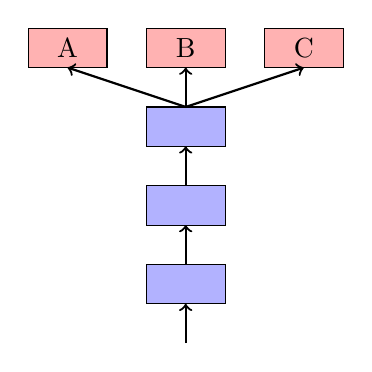
\begin{tikzpicture}
		\begin{scope} [fill opacity = .3]
		\draw [->, thick] (0,0) -- (0, 0.5);
		\draw [fill=blue, draw = black] (-0.5,1) rectangle (0.5, 0.5);
		\draw [->, thick] (0, 1) -- (0, 1.5);
		\draw [fill=blue, draw = black] (-0.5,2) rectangle (0.5, 1.5);
		\draw [->, thick] (0, 2) -- (0, 2.5);
		\draw [fill=blue, draw = black] (-0.5,3) rectangle (0.5, 2.5);
		\draw [fill=red, draw = black] (-2,4) rectangle (-1, 3.5);
		\draw [fill=red, draw = black] (-0.5,4) rectangle (0.5, 3.5);
		\draw [fill=red, draw = black] (1,4) rectangle (2, 3.5);
		\draw [->, thick] (0, 3) -- (-1.5, 3.5);
		\draw [->, thick] (0, 3) -- (0, 3.5);
		\draw [->, thick] (0, 3) -- (1.5, 3.5);
		\end{scope}
		\node at (-1.5, 3.75) {A};
		\node at (0, 3.75) {B};
		\node at (1.5, 3.75) {C};
		
		\end{tikzpicture}
	}
	\quad
	\subfloat[软共享模式]{
		\centering
		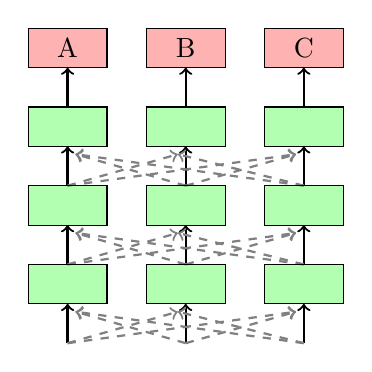
\begin{tikzpicture}
		\begin{scope} [fill opacity = .3]
		\draw [->, thick] (-1.5,0) -- (-1.5, 0.5);
		\draw [->, thick, gray, dashed] (-1.5,0) -- (-.1, 0.4);
		\draw [->, thick, gray, dashed] (-1.5,0) -- (1.4, 0.4);
		
		\draw [->, thick] (-1.5, 1) -- (-1.5, 1.5);
		\draw [->, thick, gray, dashed] (-1.5, 1) -- (-.1, 1.4);
		\draw [->, thick, gray, dashed] (-1.5, 1) -- (1.4, 1.4);
		
		\draw [->, thick] (-1.5, 2) -- (-1.5, 2.5);
		\draw [->, thick, gray, dashed] (-1.5, 2) -- (-.1, 2.4);
		\draw [->, thick, gray, dashed] (-1.5, 2) -- (1.4, 2.4);
		
		\draw [->, thick] (-1.5, 3) -- (-1.5, 3.5);
		
		\draw [fill=green, draw = black] (-2,1) rectangle (-1, 0.5);
		\draw [fill=green, draw = black] (-2,2) rectangle (-1, 1.5);
		\draw [fill=green, draw = black] (-2,3) rectangle (-1, 2.5);
		\draw [fill=red, draw = black] (-2,4) rectangle (-1, 3.5);
		
		\draw [->, thick] (0,0) -- (0, 0.5);
		\draw [->, thick, gray, dashed] (0,0) -- (-1.4, 0.4);
		\draw [->, thick, gray, dashed] (0,0) -- (1.4, 0.4);
		
		\draw [->, thick] (0, 1) -- (0, 1.5);
		\draw [->, thick, gray, dashed] (0, 1) -- (-1.4, 1.4);
		\draw [->, thick, gray, dashed] (0, 1) -- (1.4, 1.4);
		
		\draw [->, thick] (0, 2) -- (0, 2.5);
		\draw [->, thick, gray, dashed] (0, 2) -- (-1.4, 2.4);
		\draw [->, thick, gray, dashed] (0, 2) -- (1.4, 2.4);
		
		\draw [->, thick] (0, 3) -- (0, 3.5);
		
		\draw [fill=green, draw = black] (-0.5,1) rectangle (0.5, 0.5);
		\draw [fill=green, draw = black] (-0.5,2) rectangle (0.5, 1.5);
		\draw [fill=green, draw = black] (-0.5,3) rectangle (0.5, 2.5);
		\draw [fill=red, draw = black] (-0.5,4) rectangle (0.5, 3.5);
		
		\draw [->, thick] (1.5, 0) -- (1.5, 0.5);
		\draw [->, thick, gray, dashed] (1.5, 0) -- (-1.4, 0.4);
		\draw [->, thick, gray, dashed] (1.5, 0) -- (-.1, 0.4);
		
		\draw [->, thick] (1.5, 1) -- (1.5, 1.5);
		\draw [->, thick, gray, dashed] (1.5, 1) -- (-1.4, 1.4);
		\draw [->, thick, gray, dashed] (1.5, 1) -- (-.1, 1.4);
		
		\draw [->, thick] (1.5, 2) -- (1.5, 2.5);
		\draw [->, thick, gray, dashed] (1.5, 2) -- (-1.4, 2.4);
		\draw [->, thick, gray, dashed] (1.5, 2) -- (-.1, 2.4);
		
		\draw [->, thick] (1.5, 3) -- (1.5, 3.5);
		
		\draw [fill=green, draw = black] (1,1) rectangle (2, 0.5);
		\draw [fill=green, draw = black] (1,2) rectangle (2, 1.5);
		\draw [fill=green, draw = black] (1,3) rectangle (2, 2.5);
		\draw [fill=red, draw = black] (1,4) rectangle (2, 3.5);
		\end{scope}
		\node at (-1.5, 3.75) {A};
		\node at (0, 3.75) {B};
		\node at (1.5, 3.75) {C};
		
		\end{tikzpicture}
	}%
	\quad
	
	\subfloat[分层共享模式]{
		\centering
		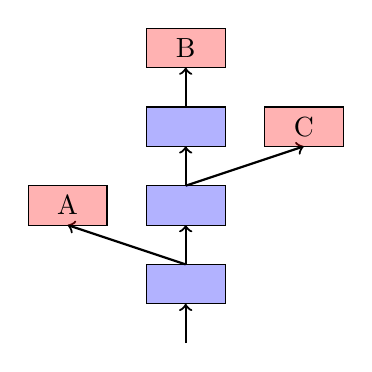
\begin{tikzpicture}
		\begin{scope} [fill opacity = .3]
		\draw [->, thick] (0,0) -- (0, 0.5);
		\draw [->, thick] (0, 1) -- (0, 1.5);
		\draw [->, thick] (0, 2) -- (0, 2.5);
		\draw [->, thick] (0, 3) -- (0, 3.5);
		\draw [->, thick] (0, 1) -- (-1.5, 1.5);
		\draw [->, thick] (0, 2) -- (1.5, 2.5);
		
		\draw [fill=blue, draw = black] (-0.5,1) rectangle (0.5, 0.5);
		\draw [fill=blue, draw = black] (-0.5,2) rectangle (0.5, 1.5);
		\draw [fill=blue, draw = black] (-0.5,3) rectangle (0.5, 2.5);
		
		\draw [fill=red, draw = black] (-0.5,4) rectangle (0.5, 3.5);
		\draw [fill=red, draw = black] (-2,2) rectangle (-1, 1.5);
		\draw [fill=red, draw = black] (1,3) rectangle (2, 2.5);
		\end{scope}
		\node at (-1.5, 1.75) {A};
		\node at (0, 3.75) {B};
		\node at (1.5, 2.75) {C};
		
		\end{tikzpicture}
	}
	\quad
	\subfloat[共享-私有模式]{
		\centering
		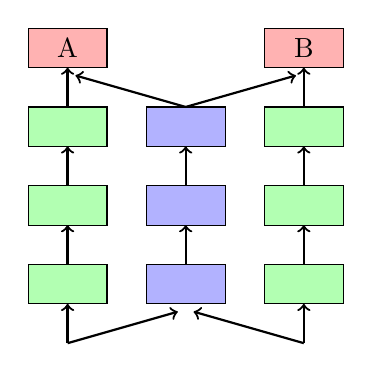
\begin{tikzpicture}
		\begin{scope} [fill opacity = .3]
		\draw [->, thick] (-1.5,0) -- (-1.5, 0.5);
		\draw [->, thick] (-1.5, 1) -- (-1.5, 1.5);
		\draw [->, thick] (-1.5, 2) -- (-1.5, 2.5);
		\draw [->, thick] (-1.5, 3) -- (-1.5, 3.5);
		
		\draw [fill=green, draw = black] (-2,1) rectangle (-1, 0.5);
		\draw [fill=green, draw = black] (-2,2) rectangle (-1, 1.5);
		\draw [fill=green, draw = black] (-2,3) rectangle (-1, 2.5);
		\draw [fill=red, draw = black] (-2,4) rectangle (-1, 3.5);
		
		\draw [->, thick] (-1.5,0) -- (-.1, .4);
		\draw [->, thick] (1.5,0) -- (.1, .4);
		\draw [->, thick] (0, 1) -- (0, 1.5);
		\draw [->, thick] (0, 2) -- (0, 2.5);
		\draw [->, thick] (0, 3) -- (-1.4, 3.4);
		\draw [->, thick] (0, 3) -- (1.4, 3.4);
		
		\draw [fill=blue, draw = black] (-0.5,1) rectangle (0.5, 0.5);
		\draw [fill=blue, draw = black] (-0.5,2) rectangle (0.5, 1.5);
		\draw [fill=blue, draw = black] (-0.5,3) rectangle (0.5, 2.5);
		
		\draw [->, thick] (1.5, 0) -- (1.5, 0.5);
		\draw [->, thick] (1.5, 1) -- (1.5, 1.5);
		\draw [->, thick] (1.5, 2) -- (1.5, 2.5);
		\draw [->, thick] (1.5, 3) -- (1.5, 3.5);
		
		\draw [fill=green, draw = black] (1,1) rectangle (2, 0.5);
		\draw [fill=green, draw = black] (1,2) rectangle (2, 1.5);
		\draw [fill=green, draw = black] (1,3) rectangle (2, 2.5);
		\draw [fill=red, draw = black] (1,4) rectangle (2, 3.5);
		\end{scope}
		\node at (-1.5, 3.75) {A};
		\node at (1.5, 3.75) {B};
		
		\end{tikzpicture}
	}
	
	\caption{多任务学习的几种常见共享模式}
	\label{fig:mtl_archs}
\end{figure}

\section{自然语言处理}
\label{sec:nlp}





\section{多任务自然语言处理}
\label{sec:mtl4nlp}

\chapter{模型}
\label{cha:model}

\section{Transformer}
\label{sec:tf}

\section{多任务Transformer}
\label{sec:mtl_tf}

\subsection{S-P结构}

\subsection{S-C结构}

\subsection{L-I结构}

\subsection{L-E结构}

\section{实现细节}
\label{sec:imp}
\chapter{实验}
\label{cha:exp}
本章介绍验证模型结构所进行的实验。首先,使用Transformer作为基线模型实验了单任务学习下的模型性能,接着使用相同的超参设定实验了~\ref{sec:mtl_tf}~节介绍的四种多任务Transformer的性能。具体地,在第~\ref{sec:task}~节介绍实验任务,在第~\ref{sec:ds}~节介绍数据集相关信息,在第~\ref{sec:results}~节介绍实验结果。最后,~\ref{sec:analysis}~节给出了实验分析。

\section{任务描述}
\label{sec:task}
我们在\emph{文本分类}(Text Classification)这一经典NLP任务上进行实验。事实上,很多NLP问题都可以归为文本分类的范畴,例如情感分析(Sentiment Analysis, SA)、自然语言推理(Natural Language Inference, NLI)等。在目前被广泛使用的多任务基准数据集GLUE\cite{DBLP:conf/emnlp/WangSMHLB18}中,所有任务都可以被归为文本分类任务。

文本分类即将一段文本归到某个特定的预先定义的类别。待分类的文本通常是一个句子(如情感分析)或一个句子对(如自然语言推理)。需要注意的是,这里的一个句子并不一定是常规意义上以一个句号为结束标识符的一句话,也有可能包含多句话。文本分类任务在现实生活中有着广泛的应用,如自动分析产品评价、微博情感分析、文档归类等等。文本分类任务需要模型能够抽取出易于分类的句子表示,即需要句子级的文本表示模型。

具体地,本文在情感分析任务上进行实验:对于一段用户生成的文本,模型需要判断其情感极性为正向还是负向。然而对于不同领域的文本通常需要关注不同的特征,例如在食物类的评论文本中模型应当更加关注“好吃”、“美味”等词,而在电影评论文本中应当更加关注“好看”、“烂片”等词语。同时,不同领域的文本分类任务常常也需要某些通用的特征,如“很棒”、“失望”等词在所有与情感倾向有关的分类任务中都是应当被关注的。而事实上,在某个特定的领域内,文本数据量常常是有限的,这种情况下单任务学习通常难以取得很好的效果,可以通过多任务学习来利用其他领域的相关知识帮助分类。

\section{数据集}
\label{sec:ds}
我们的基线单任务模型以及多任务模型在16个文本分类数据集上进行了对比实验,其中的前14个数据集来自亚马逊的产品评论\footnote{\url{https://www.cs.jhu.edu/˜mdredze/datasets/ sentiment/}},但是来自各自不同的领域,如图书、电子、光盘等。该部分数据由Blitzer等人\cite{DBLP:conf/acl/BlitzerDP07}收集而成,其余两个数据集IMDB\cite{DBLP:conf/acl/MaasDPHNP11}和MR\cite{DBLP:conf/acl/PangL05}则来自电影评论。每个数据集包含约2000个样本,其中70\%划分为训练集,10\%划分为验证集,20\%划分为测试集。数据集的具体统计信息见表~\ref{tb:dataset}。

\begin{table}[htb]
	\centering
	\caption{数据集统计数据}
	\begin{tabular}{ccccccc}
		\toprule[2pt]
		数据集&训练集大小&验证集大小&测试集大小&类别数&平均长度&词表大小\\
		\midrule[1pt]
		Books& 1400& 200& 400& 2& 159& 19K\\
		Elec& 1398& 200& 400& 2& 101& 11K\\
		DVD& 1400& 200& 400& 2& 173& 20K\\
		Kitchen& 1400& 200& 400& 2& 89& 9K\\
		Apparel& 1400& 200& 400& 2& 57& 7K\\
		Camera& 1397& 200& 400& 2& 130& 9K\\
		Health& 1400& 200& 400& 2& 81& 9K\\
		Music& 1400& 200& 400& 2& 136& 17K\\
		Toys& 1400& 200& 400& 2& 90& 10K\\
		Video& 1400& 200& 400& 2& 156& 17K\\
		Baby& 1300& 200& 400& 2& 104& 8K\\
		Mag& 1370& 200& 400& 2& 117& 11K\\
		Soft& 1315& 200& 400& 2& 129& 11K\\
		Sports& 1400& 200& 400& 2& 94& 10K\\
		IMDB& 1400& 200& 400& 2& 269& 25K\\
		MR& 1400& 200& 400& 2& 21& 7K\\
		\bottomrule[2pt]
	\end{tabular}
	\label{tb:dataset}
\end{table}

数据集中的部分样本可见表~\ref{tb:examples}。
\begin{table}[htb]
\centering
\caption{数据集中的部分样本}
\begin{tabular}{cc}
\toprule[2pt]
领域&样例\\
\midrule[1pt]
Books&blabla...\\
Mag&blabla...\\
\bottomrule[2pt]
\end{tabular}
\label{tb:examples}
\end{table}
\section{实验结果}
\label{sec:results}
实验结果如表~\ref{tb:results}~所示,我们的四个多任务模型在十六个文本分类任务上均超过了单任务训练的表现,验证了多任务学习在Transformer上的有效性。其中,L-I结构在四种多任务架构中表现最好,S-P结构表现最差。L-I结构和L-E结构取得的较好结果表明,在每一层都形成任务特定表示的做法相比在网络的顶层获取特征更为合理。同时,注意到S-C结构也能达到较好的准确率,这也肯定了之前被广泛使用的硬共享模式的效果,但随着任务之间差异性的增大,我们有理由认为L-I和L-E的共享架构相比传统架构将表现出更大的优越性。

\begin{table}[htb]
	\centering
	\caption{模型在测试集上的分类准确率}
	\begin{tabular}{c|cccccc}
		\toprule[2pt]
		\multirow{2}*{数据集}&\multirow{2}*{单任务}&\multicolumn{4}{c}{多任务}\\
		\cline{3-6}
		&&S-P结构& S-C结构& L-I结构& L-E结构\\
		\midrule[1pt]
		Books& 83.50& 82.50& 84.00& 85.00& 84.50\\
		Elec& 79.50& 82.50& 83.50& 84.75& 85.75\\
		DVD& 82.75& 84.50& 85.50& 85.75& 85.75\\
		Kitchen& 79.50& 83.50& 85.00& 89.00& 87.75\\
		Apparel& 82.75& 85.50& 86.75& 86.00& 85.75\\
		Camera& 81.75& 84.25& 85.00& 87.00& 89.00\\
		Health& 86.00 & 85.50& 87.50& 88.00& 86.75\\
		Music& 76.50& 83.00& 83.00& 82.75& 81.50\\
		Toys& 80.00& 84.75& 86.25& 88.25& 86.50\\
		Video& 84.75& 81.25& 85.50& 86.50& 84.25\\
		Baby& 81.00 &87.75& 85.50& 87.25& 87.50\\
		Mag& 89.00& 85.00& 91.00& 89.75& 89.25\\
		Soft& 86.50& 86.00& 88.75& 86.50& 87.75\\
		Sports& 80.25& 84.25& 83.75& 86.00& 85.50\\
		IMDB& 80.75& 84.75& 85.00& 84.50& 84.50\\
		MR& 75.25& 76.00& 75.75& 78.00& 76.50\\
		\rowcolor{lightgray}
		AVG.& 81.86& 83.81& 85.11& \textbf{85.94}& 85.53\\
		\bottomrule[2pt]
	\end{tabular}
	\label{tb:results}
\end{table}

在实践中,神经网络的层数通常是一个比较重要的超参数,模型性能有时会由于层数的不同而产生较大差异。之前的实验中使用的模型均为4层Transformer,为探究多任务Transformer结构对网络层数的敏感性,我们实验了四种结构在不同层数下的平均分类准确率,结果如图~\ref{fig:layer_dis}~所示。

可见,在各个层数设定中,逐层共享结构(L-I结构和L-E结构)均优于传统的硬共享结构(S-P结构和S-C结构),且L-I结构在三种设定中都取得了最优准确率,这一实验结果证明了模型的鲁棒性。

\begin{figure}[htb]
\centering
\begin{tikzpicture}
\begin{axis}[
	xlabel={层数},
	ylabel={准确率},
	legend style={
		cells={anchor=east},
		legend pos=outer north east,
	}
]

\addplot coordinates{
	(2, 0.8547)
	(4, 0.8594)
	(6, 0.8523)
};

\addplot coordinates{
	(2, 0.8539)
	(4, 0.8553)
	(6, 0.8500)
};

\addplot [mark=x]coordinates {
	(2, 0.8451)
	(4, 0.8381)
	(6, 0.8167)
};

\addplot coordinates{
	(2, 0.8484)
	(4, 0.8511)
	(6, 0.8478)
};
\legend{L-I结构,L-E结构,S-P结构,S-C结构}
\end{axis}
\end{tikzpicture}
\caption{网络层数对测试集准确率的影响}
\label{fig:layer_dis}
\end{figure}

\section{实验分析}
\label{sec:analysis}

\begin{figure}[htb]
\centering
\includegraphics[scale=0.4]{L-E-attn.png}
\caption{L-E结构注意力可视化}
\label{fig:l-e-attn}
\end{figure}
\chapter{总结与展望}
\label{cha:conclusions}

%%%%%%%%%%%%%%%
%% 论文后置部分
%%%%%%%%%%%%%%%
\backmatter

%% 插图索引
% \listoffigures
%% 表格索引
% \listoftables

%% 致谢

\begin{acknowledgments}

  四载匆匆,倏忽而至,终于要毕业了。
  
  我还清楚地记得那段穿着军装、踢着正步、烈日永远不会缺席的时光,记得敲下第一行\texttt{Hello World}时的懵懂,也还记得和队友们一起通宵做数模的疲惫,更记得无数个平凡的日子里坐在教室里一起听课的同学们和站在讲台上的教授们……一切仿佛就在昨日,如今却要离开这里了。
  
  回首这段岁月,我只觉得幸运。何其幸运,能遇到这么多学识渊博、兢兢业业的老师;何其幸运,能遇到这么多优秀又谦虚的同学们。借此机会,我想向你们致以真挚的感谢。
  
  首先,我想感谢本文的指导老师,也即将是我博士阶段的导师:邱锡鹏老师和黄萱菁老师。没有他们提供的悉心指导和实验环境,就不会有这篇文章。另外,还要特别感谢邱老师,他的学术品位、研究热情和为人方式都激励着我,我相信我也将度过同样充实且舒适的博士生涯。
  
  然后,我要感谢本科阶段给予我巨大帮助的老师们和同学们。感谢陈慧婵老师和郭艳艳老师,他们为我打下了扎实的数理基础;感谢张淑平老师、张立勇老师和顾新老师,让我掌握了必要的专业知识;感谢周水生老师,在我参与数模期间提供了大量指导。感谢一路同行的同学们,王磊、余天焕、徐之浩、班浩等等,你们一直是我成长路上的榜样;还要感谢陪伴我四年的室友,王敏锐、王许丞和冯尧,感谢你们一直以来的包容与帮助。
  
  最后,我要感谢我的家人。感谢我的父母,在我的求学路上面临的每一次选择,你们都给予了最大的鼓励与信任,没有你们一如既往的支持,也不会有现在的我;还要感谢我的女朋友曲雪纯,遇到你是我本科阶段最大的收获之一。你们一直,也将永远是我的最强大的后盾!
  
  \begin{flushright}
  	\emph{孙天祥}\\
  	二零一九年六月于西电
  \end{flushright}

\end{acknowledgments}



% 参考文献
\bibliographystyle{gbt7714-2005}
\bibliography{refs}

\end{document}
